\documentclass[a4paper, 12pt, final, garamond]{book}
\usepackage{cours-preambule}

\titleformat{\item}{}{\arabic{item})}{.5em}{}{}
\titleformat{\subitem}{}{\arabic{item}) \alph{subitem} --}{.5em}
{}{}

\makeatletter
\renewcommand{\@chapapp}{Devoir surveill\'e -- num\'ero}
\makeatother

\begin{document}
\setcounter{chapter}{7}

\chapter{Commentaires sur le DS n\degree8}

\begin{NCprop}[width=\linewidth]{\centering\bfseries\ Rappel des malus}
    Chacune des lettres suivantes sur vos copies sont des malus de \num{1}
    point.\smallbreak
    \begin{minipage}{0.50\linewidth}
        \begin{itemize}
            \item A~: application numérique mal faite~;
            \item Q~: question mal ou pas indiquée~;
            \item P~: nom/prénom non indiqué~;
        \end{itemize}
    \end{minipage}
    \begin{minipage}{0.50\linewidth}
        \begin{itemize}
            \item U~: unité manquante ou mauvaise~;
            \item H~: homogénéité non respectée~;
            \item S~: chiffres significatifs non respectés~;
        \end{itemize}
    \end{minipage}
\end{NCprop}

\section{Commentaires généraux}

DS à 46, assez réussi. Note moyenne à 11/20. Total malus~: \textbf{81},
relativement bas. Par contre, \textbf{beaucoup de malus -U}~: un potentiel
\textbf{s'exprime en volts}~! On compte 1 seule personne sans un seul malus,
pour un total de \textbf{1} point de bonus. Plus grand gain de place par rapport
au DS07~: 27. Plus grande perte de place~: -23 places. Vous noterez que
\textbf{tous les exercices sont tirés de vrais sujet de 2022}~: ce que vous
venez de faire est proche de ce que vous aurez dans \SI{12}{mois}.

Remarques générales~:
\begin{enumerate}
  \item Les équations bilans \textbf{ne peuvent avoir d'électrons}~!
  \item Pensez aux \textbf{phases} dans les équations.
  \item $K$ est égal au quotient réactionnel \textbf{à l'équilibre}.
  \item Une molécule \textbf{n'a pas un nombre d'oxydation} mais une
    \textbf{charge}.
  \item Justifier l'ordre des domaines par \textbf{n.o. croissant}.
  \item Il faut connaître la \textbf{définition} du \textbf{produit de
    solubilité}~: dissociation du solide en ses \textbf{composés ioniques}, sans
    autres éléments (\ce{H2O} par exemple).
\end{enumerate}

\begin{center}
    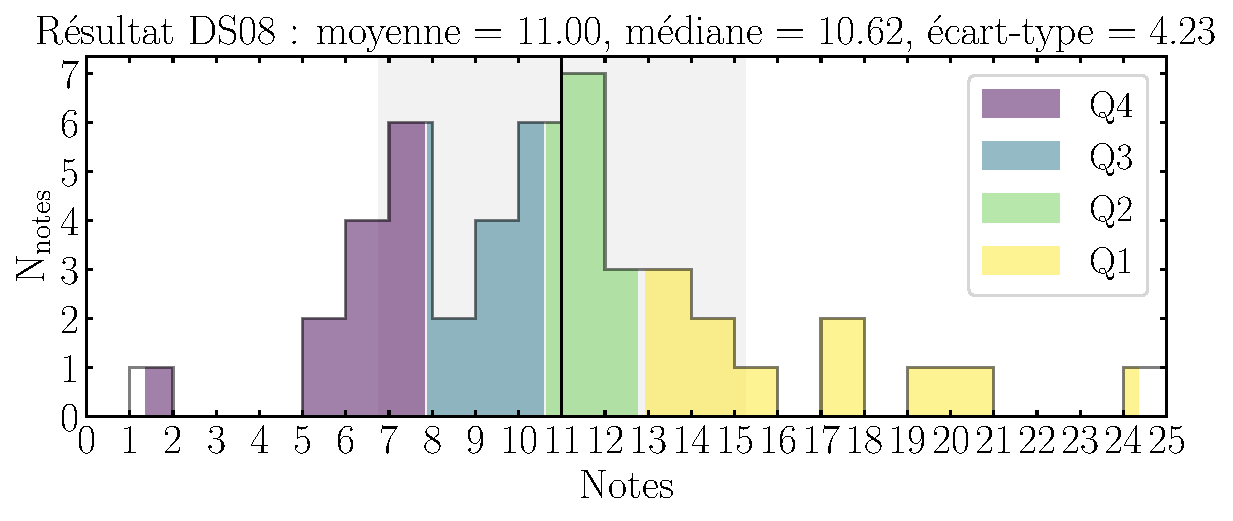
\includegraphics[width=.8\linewidth]{res_DS08.pdf}
\end{center}
\vspace*{-20pt}

\section{Exercice 1 \hfill \textcolor{red}{/22}}
\begin{enumerate}
  \item Penser aux phases.
    \hfill \textcolor{ForestGreen}{/2}
  \item Une densité n'a pas d'unité.
    \hfill \textcolor{red}{/8}
  \item Justification $\neq$ «~on lit les couples sur la figure~»~: anode =
    oxydation, cathode = réduction, qui est l'oxydant du couple (analyse n.o. ou
    écriture des demi-équations).
    \hfill \textcolor{ForestGreen}{/6}
  \item RAS sur toute la fin.
\end{enumerate}

\section{Exercice 2 \hfill \textcolor{red}{/49}}
\begin{enumerate}
  \item Attention aux puissances et aux coefficients stœchiométriques.
    \hfill \textcolor{ForestGreen}{/4}
  \item Le fonctionnement du titrage n'a pas été compris, ou la question
    «~donner l'équation du titrage~» complètement oubliée. Un schéma de titrage
    doit être complet. On rajoute de l'eau pour \textbf{négliger la dilution}.
    \hfill \textcolor{ForestGreen}{/6}
  \item Analyse et logique.
    \hfill \textcolor{ForestGreen}{/6}
  \item RAS.
    \hfill \textcolor{ForestGreen}{/5}
  \item Ne pas oublier la puissance 2.
    \hfill \textcolor{ForestGreen}{/4}
  \item Les questions de calcul de $K$ valent beaucoup de point. Il faut bien
    intérgrer la méthode de calcul. Notamment, \textbf{écrire la constante
    d'équilibre} que vous cherchez dès l'obtention de l'équation bilan.
    \hfill \textcolor{ForestGreen}{/15}
  \item Question pas traitée. Faite en TP la veille… dommage.
    \hfill \textcolor{ForestGreen}{/5}
\end{enumerate}

\section{Exercice 3 \hfill \textcolor{red}{/53}}
\begin{enumerate}
  \item Justifier la construction, même ce qui n'est pas explicitment demandé
    dans la question. TB réussi sinon.
    \hfill \textcolor{ForestGreen}{/10}
  \item \textbf{Ne pas se tromper sur la définition de $\mathbf{K_s}$~!} Et non,
    on n'a pas $\pH = \mathrm{p}K_s$ à la frontière…
    \hfill \textcolor{ForestGreen}{/6}
  \item La hauteur d'une frontière \textbf{dépend de la convention de tracé}~!
    On n'a pas automatiquement $E\degree = E$.
    \hfill \textcolor{ForestGreen}{/5}
  \item Même commentaire qu'exercice 2 question 7. Cependant, \textbf{vous ne
    pouvez pas dire «~comme pour l'exercice 2~»}~: les exercices sont notés
    \textit{indépendemment}.
    \hfill \textcolor{ForestGreen}{/13}
  \item Justifier $\pH = \mathrm{p}K_a$.
    \hfill \textcolor{ForestGreen}{/4}
  \item RAS.
    \hfill \textcolor{ForestGreen}{/8}
  \item Question du TD.
    \hfill \textcolor{ForestGreen}{/7}
\end{enumerate}

\section{Problème \hfill \textcolor{red}{/46}}
\begin{enumerate}
  \item Question type problème~: il faut savoir traduire ce que veut dire «~il
    se forme du tartre~», comprendre les conditions de réalisation, les données
    disponibles et ce qu'il faut déduire.
    \hfill \textcolor{ForestGreen}{/10}
  \item RAS.
    \hfill \textcolor{ForestGreen}{/2}
  \item Lisez bien les données~: si $\mathrm{p}K_a$ est donné, alors $K_a$ se
    trouve de manière instantanée (à condition de \textbf{connaître la
    définition de $K_a$})~!
    \hfill \textcolor{ForestGreen}{/2}
  \item Question plus compliquée que $\pH = \mathrm{p}K_a + \log
    \frac{[\ce{A-}]}{[\ce{AH}]}$.
    \hfill \textcolor{ForestGreen}{/7}
  \item Pensez aux diagrammes en $\mathrm{p}K_a$ pour synthétiser les espèces en
    présence.
    \hfill \textcolor{ForestGreen}{/4}
  \item Revoir la notion de pression partielle.
    \hfill \textcolor{ForestGreen}{/7}
  \item Simple utilisation de la loi de \textsc{Duperray}.
    \hfill \textcolor{ForestGreen}{/2}
  \item RAS sur toute la fin.
\end{enumerate}

\end{document}
